\documentclass[12pt]{article}

\usepackage[utf8]{inputenc}
\usepackage{amsmath}
\usepackage{graphicx}
\usepackage{geometry}
\geometry{a4paper, margin=1in}

\renewcommand{\thefigure}{S\arabic{figure}}

\title{Supplementary material for \\ \textit{Dynamic consequences of declining vaccination coverage in a heterogeneous world}}
\author{Emily Howerton, Ayesha Mahmud, David J.D. Earn, \\Bryan T. Grenfell, C. Jessica E. Metcalf}

\date{}

\begin{document}

\maketitle


\section{Theoretical honeymoon time in the SIR model}
We consider  here how reductions in vaccination can lead to rebounds in disease prevalence in a SIR (Susceptible, Infected, Recovered) model. In particular, we will focus on the post-vaccination ``honeymoon", or how long it takes for the disease to rebound after vaccination starts declining. Note, we use the term ``immunization" thorughout to account for both vaccination coverage and imperfect vaccine efficacy (i.e., immunization represents those successfully immunized, not merely vaccinated). 

To begin, we will consider the simplest case where (a) a population has been under a ``pre-decline'' vaccination regime for a sufficiently long period of time to be at equilibrium, and (b) that the pathogen is locally eliminated.  Let $v_0$ be the immunization rate during the period of herd immunity, and let $v$ be the immunication rate after the decline begins. 

In the SIR model, we know there are two possible equilibria: 
\begin{enumerate}
    \item disease-free equilibrium, where $S^* = v_0$
    \item endemic equilibrium, where $S^* = \frac{1}{\beta}(\mu + \gamma + \frac{\mu(\mu + \gamma)}{\sigma})$
\end{enumerate}

Here, we only consider the first case where a population is above the herd immunity threshold, $1/R_0$, because otherwise there is no honeymoon period. We are interested in the duration of the honeymoon period, which we hypothesize will depend on a number of factors including the $R_0$ of the pathogen, the equilibrium number of susceptibles $S^*$, the birth rate $\mu$, the immunization rate $v$ under decline, and the timing of importations. Because we cannot control the timing of importations, we define the honeymoon period as the time it takes for $R_e = R_0 \cdot S(t) > 1$. In other words, the time it takes for $R_e$ to cross 1 is a lower bound on the honeymoon period, where any importation after this point will start an outbreak. 

We can calculate analytically the time it takes for $R_e$ to cross 1, under assumptions of local extinction (i.e., $I = 0$) and a constant post-decline immunization rate, $v$. In this case, we have a differential equation for the number of susceptibles, $S$, which we can solve using the following steps:

\begin{align*}
    \frac{dS}{dt} &= \mu (1-v) - \mu S \\
    e^{\mu t}\Big(\frac{dS}{dt} + \mu S \Big) &= e^{\mu t} \mu (1-v) \\
    \int e^{\mu t}\Big(\frac{dS}{dt} + \mu S \Big) dt &= \int e^{\mu t} \mu (1-v) dt \\
    \int e^{\mu t}\frac{dS}{dt} + e^{\mu t}\mu S dt &= \int e^{\mu t} \mu (1-v) dt \\
    e^{\mu t} S &= (1-v) e^{\mu t} + C \\
    S(t) &= (1-v) + C e^{-\mu t}
\end{align*}

\noindent
and solving $S_0 = (1-v) + C e^{-\mu \cdot 0}$ gives us $C = S_0 - (1-v)$.
Thus, we have:

$$
S(t) = (1-v) + (S_0 - (1-v)) e^{-\mu t}
$$

\noindent
We can then find the time $t$ at which $R_e = R_0 S(t) = 1$, which yields

% \begin{align}
%     (1-v) + (S_0 - (1-v)) e^{-\mu t} &= 1/R_0  \\
%     (S_0 - (1-v))e^{-\mu t}  &= (1/R_0 - (1-v)) \\\
%     e^{-\mu t}  &= \frac{1/R_0 - (1-v)}{S_0 - (1-v)} \\
% \end{align}
$$
t = \frac{-1}{\mu} \log \Big(\frac{1/R_0 - (1-v)}{S_0 - (1-v)}\Big)
$$

\noindent
We can also rewrite this equation to show us the relationship between pre- and post-decline immunization levels that yield equivalent honeymoon periods. When vaccination rates are above the herd immunity threshold, $S_0 = 1-v_0$ is the pre-drop vaccination coverage, so 

% \begin{align}
%     t &= \frac{-1}{\mu} \log \Big(\frac{1/R_0 - (1-v)}{(1-v_0) - (1-v)}\Big) \\
%     - t \mu &= \log \Big(\frac{1/R_0 - (1-v)}{(1-v_0) - (1-v)}\Big) \\
%     e^{- t \mu} &= \Big(\frac{1/R_0 - (1-v)}{(1-v_0) - (1-v)}\Big) \\
%     (1-v_0) - (1-v) &= e^{t \mu} (1/R_0 - (1-v)) \\
%     v - v_0 &= e^{t \mu} (v - 1 + 1/R_0) \\
%     v_0 &= v - e^{t \mu} (v - 1 + 1/R_0) \\
%     v_0 &= v(1 - e^{t \mu}) + e^{t \mu} (1 - 1/R_0)
% \end{align}

$$
t = \frac{-1}{\mu} \log \Big(\frac{1/R_0 - (1-v)}{(1-v_0) - (1-v)}\Big)
$$

\noindent
which can be simplified to
$$
v_0 = v(1 - e^{t \mu}) + e^{t \mu} (1 - 1/R_0).
$$

\section{Age-structured model}
Our age-structured model defines a discrete set of $A$ age classes.  Transmission between individuals of different age classes is governed by a who-acquires-infection-from-whom (WAIFW) matrix, $\theta_{i,j}$, where $i$ and $j$ index age classes. The full system of ordinary differential equations is as follows:

\begin{align*}
    % susceptible 
    \frac{dS_{i=1}}{dt} &= \mu (1-v) - \sum_{j=1}^{A} \theta_{1,j} S_1 I_j - \mu S_1 - \alpha_1 S_1 \\
    \frac{dS_{i\neq1}}{dt} &= \alpha_{i-1} S_{i-1} - \sum_{j=1}^{A} \theta_{i,j} S_i I_j - \mu S_i - \alpha_i S_i \\
    % infected
    \frac{dI_{i=1}}{dt} &= \sum_{j=1}^{A} \theta_{1,j} S_1 I_j - (\gamma + \mu) I_1 - \alpha_1 I_1 \\
    \frac{dI_{i\neq1}}{dt} &= \alpha_{i-1} I_{i-1} + \sum_{j=1}^{A} \theta_{i,j} S_i I_j - (\gamma + \mu) I_i - \alpha_i I_i \\
    % recovered
    \frac{dR_{i=1}}{dt} &= \mu v + \gamma I_1 - \mu R_1 - \alpha_1 R_1 \\
    \frac{dR_{i\neq1}}{dt} &= \alpha_{i-1} R_{i-1} + \gamma I_i - \mu R_i - \alpha_i R_i 
\end{align*}

\noindent
where $\alpha_i$ is the rate of aging out of age class $i$, $\mu$ is the birth and death rate, $\gamma$ is the recovery rate, $v$ is the immunization rate. This model assumes a total population size of 1, and compartments represent the proportion of individuals in each age class.

We can calculate the basic reproduction number, $R_0$, and the effective reproduction number, $R_e$, for this model using the Next Generation Matrix method. In this case, the next generation matrix, $K$, is given by 

$$
    K = \frac{1}{\gamma + \mu} \begin{bmatrix}
     \theta_{1,1} S_1(t) & \theta_{1,2} S_1(t) & \cdots & \theta_{1,n} S_1(t) \\
    \theta_{2,1} S_2(t) & \theta_{2,2} S_2(t) & \cdots & \theta_{2,n} S_2(t) \\
    \vdots & \vdots & \ddots & \vdots \\
    \theta_{n,1} S_n(t) & \theta_{n,2} S_n(t) & \cdots & \theta_{n,n} S_n(t) \\
    \end{bmatrix} = \frac{1}{\gamma + \mu} \theta \overrightarrow{S(t)},
    $$

\noindent
for which we calculate the dominant eigenvalues numerically.

% To calculate $R_0$ in the age-structured model, we use the Next Generation Matrix (NGM) method outlined in Diekmann et al 1990. To do so, we follow the steps from the Bjornstad book:
% \begin{enumerate}
%     \item Define the infected states, $X = (I_1, I_2, ..., I_n)$ for ages $i = 1, 2, ..., n$
%     \item Define the new infection terms, $\mathcal{F}(X) = \Big[ \sum_{j=1}^{n} \theta_{i,j} I_j S_i  \Big]$ for ages $i = 1, 2, ..., n$
%     \item Define all losses out of infected states, $\mathcal{V}^-(X) = \Big[ (\gamma + \mu) I_i \Big]$ repeated for all ages.
%     \item Define all gained transfers between infected states, $\mathcal{V}^+(X) = \Big[ 0 \Big]$ repeated for all ages.
%     \item Define the total losses out of infected states, $\mathcal{V}(X) = \mathcal{V}^-(X) - \mathcal{V}^+(X) = \Big[ (\gamma + \mu) \Big]$.
%     \item Compute the jacobians of $F$ and $V$. We do not evaluate at the disease-free equilibrium, because we will also use this  evaluated at to calculate $R_t$. The jacobian of $V$, $v = \Big[\frac{\partial \mathcal{F}_i}{\partial X_j}\Big]$, will be $v = (\gamma + \mu)$ along the diagonal and zero elsewhere.  
%     The jacobian of $F$ is
%     $$
%     f = \Big[\frac{\partial \mathcal{F}_i}{\partial X_j}\Big] =  \begin{bmatrix}
%      \theta_{1,1} S_1 & \theta_{1,2} S_1 & \cdots & \theta_{1,n} S_1 \\
%     \theta_{2,1} S_2 & \theta_{2,2} S_2 & \cdots & \theta_{2,n} S_2 \\
%     \vdots & \vdots & \ddots & \vdots \\
%     \theta_{n,1} S_n & \theta_{n,2} S_n & \cdots & \theta_{n,n} S_n \\
%     \end{bmatrix}
%     $$
%     \item Compute the next generation matrix, $K = f v^{-1}$. Because $v$ is diagnoal, then $v^{-1}$ is another diagonal matrices with elements $1/(\gamma + \mu)$. Then, $R_0$ is the largest eigenvalue of $K$, evaluated at the disease-free equilibrium (or with $S(t)$ for $R_t$).
% \end{enumerate}

\section{Unity beta calculation}
To quantify the role of age-structured dynamics, we will use a theoretical quantity called ``unity beta". Consider an age-structured transmission process that is governed by heterogeneous contacts between age groups, where the number of new infections in the age structured model is

$$
\text{age-structured infections} =  \frac{1}{N}\sum_{i=1}^{n}\sum_{j=1}^{n} \theta_{i,j} S_i I_j
$$

\noindent
where $\theta_{i,j}$ is the transmission rate between age groups $i$ and $j$. We can then calculate a time-varying quantity, $\hat{\beta}(t)$, called ``unity beta" that ensures the number of new infections in the age-structured model is equal to the number of new infections in a non-age-structured model, where 

\begin{align*}
    \text{age-structured infections} &=  \frac{1}{N}\sum_{i=1}^{n}\sum_{j=1}^{n} \theta_{i,j} S_i I_j \\
    &= \frac{\hat{\beta}(t)}{N}\sum_{i=1}^{n} S_i \sum_{j=1}^{n} I_j \\
    &= \text{homogenous infections}
\end{align*}

\noindent
given that 

$$
\hat{\beta}(t) = \frac{\sum_{i=1}^{n}\sum_{j=1}^{n} \theta_{i,j} S_i I_j}{\sum_{i=1}^{n}S_i\sum_{j=1}^{n}I_j}
$$

\noindent
This ratio can be interpreted as the ratio of the number of new infections in the age-structured model to the number of new infections in the homogenous model. If $\hat{\beta}(t) > 1$ then age-structured dynamics are fast relative to the homogenous dynamics, and vice versa if $\hat{\beta}(t) < 1$.

% In this case, however, the homogeneous model transmission rate is determined by $k(t)$, where the transmission rate becomes the value that is necessary to generate the same dynamics as the age-structured model. However, such dynamics can yield different reproduction numbers, so we may also be interested in the relationship between age-structured and homogenous dynamics when fixing the reproduction number. This is the case we use for the main text analysis. 

% In particular, we contrast a number of WAIFW matrices, which on their own have different basic reporduction numbers. Thsu, to enable comparison, we calculate a scalar $c$ such that the reproduction number yields a given $R_0 = \beta/\gamma$. In the main text, we use $R_0 = 17$. Thus, we have

% \begin{align}
%     \text{age-structured infections} &=  \frac{c}{N}\sum_{i=1}^{n}\sum_{j=1}^{n} \theta_{i,j} S_i I_j \\
%     \text{homogenous infections} &=  \frac{\beta}{N}\sum_{i=1}^{n} S_i \sum_{j=1}^{n} I_j
% \end{align}

% \noindent
% Following the same approach, we can equate these two quantities with a ratio $k(t)$: 

% \begin{align}
%     \frac{c}{N}\sum_{i=1}^{n}\sum_{j=1}^{n} \theta_{i,j} S_i I_j &= \frac{k(t)\beta}{N}\sum_{i=1}^{n} S_i \sum_{j=1}^{n} I_j
% \end{align}

% \noindent
% where

% \begin{align}
%     k(t) = \frac{c\sum_{i=1}^{n}\sum_{j=1}^{n} \theta_{i,j} S_i I_j}{\beta\sum_{i=1}^{n} S_i \sum_{j=1}^{n} I_j}
% \end{align}

% \noindent
% This quantity, $k(t)$ only differs slightly from the previous definition of unity beta, $\hat{\beta}(t)$, where it is the scaled ratio of the number of new infections in the homogenous model to the number of new infections in the age-structured model with an equivalent transmission rate. Interpretation is the same as $\hat{\beta}(t)$ above.

\section{Metapopulation model}

We consider a metapopulation model with $P$ identical patches that are assumed to be equally connected, such that $c\%$ of transmission arises from cross-patch contact. The model can be defined as 

\begin{align*}
    \frac{dS_p}{dt} &= \mu (1-v_p) - \beta \sum_{q=1}^{P} C_{p,q} S_p I_q - \mu S_p \\
    \frac{dI_p}{dt} &= \beta \sum_{q=1}^{P} C_{p,q} S_p I_q - (\gamma + \mu) I_p \\
    \frac{dR_p}{dt} &= \mu v_p + \gamma I_p - \mu R_p
\end{align*}

\noindent
where $C_{p,q}$ is the connectivity matrix, which has $1-c$ along the diagonal and $c/(P-1)$ elsewhere. Analagous to the age-structured case, the next generation matrix is given by 
$$
    K = \frac{\beta}{\gamma + \mu} C \overrightarrow{S(t)},
$$
where $\overrightarrow{S(t)}$ is the number of susceptibles in each patch at time $t$. We specify immunization levels to drop in $\rho \%$ of these patches and the others remain at pre-decline levels. 

\pagebreak

\section{Supplementary Figures}

% \begin{figure}[h]
%     \centering
%     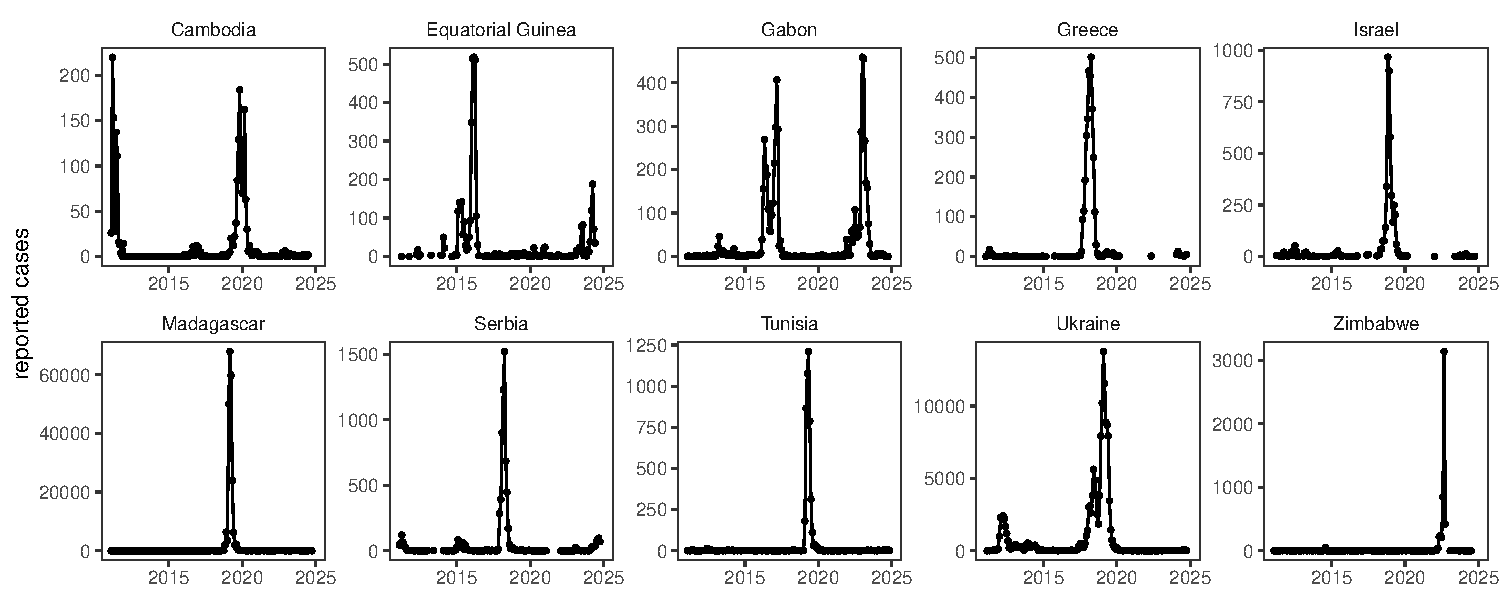
\includegraphics[width=\textwidth]{honeymoon_examples.pdf}
%     \caption{ADD HERE}
% \end{figure}

\begin{figure}[h]
    \centering
    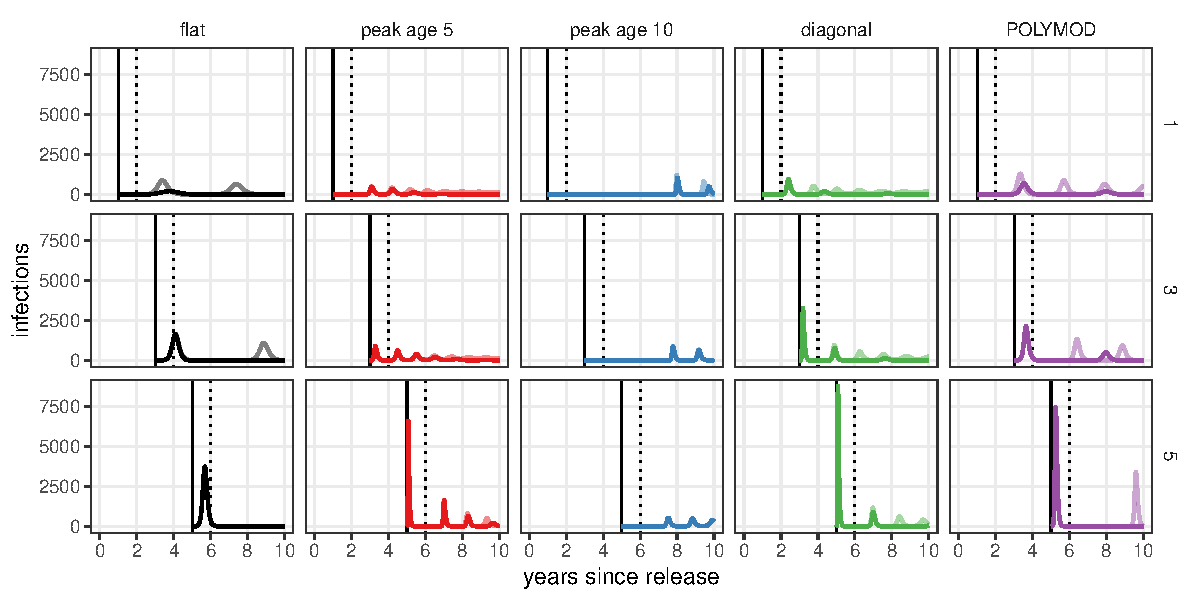
\includegraphics[width=\textwidth]{introduction_timing.pdf}
    \caption{Sensitivity of results to the timing of infection introduction. For each WAIFW matrix (columns, see main text), simulated dynamics when a single infection is introduced into the 5 year old age class 1, 3, or 5 years after the drop in immunization (rows). The solid vertical line shows the timing of introduction. The lighter line shows simulation results if immunization returns to pre-decline levels 1 year after the drop (shown by dotted line).}
\end{figure}

\begin{figure}[h]
    \centering
    
\includegraphics[width=\textwidth]{honeymoon_age_full_comparestart.pdf}
    \caption{Theoretical honeymoon time predictions, computed as time until Re > 1, under five assumptions about age-structured mixing. Results are shown for a population with $\mu =1/80 \text{ years}^{-1}$, a pathogen with $R_0 = 17$, and a pre-decline immunization of 95\% and 96\%. 
}
\end{figure}

\begin{figure}[h]
    \centering
    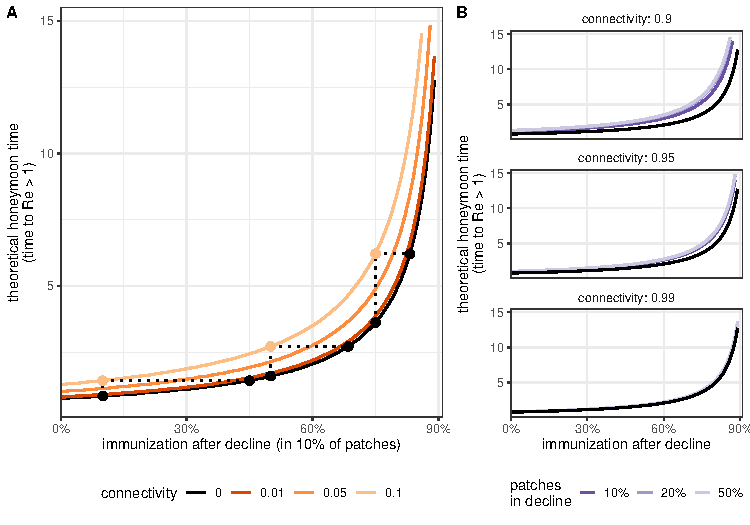
\includegraphics[width=\textwidth]{connectivity_fig.pdf}
    \caption{Role of patch connectivity in theoretical honeymoon time. (A) Theoretical honeymoon time, computed as time until Re > 1, by post-decline immunization when drops occur in 10\% of patches among an equally connected network. Line color shows connectivity between patches (where 0.05 indicates 5\% of transmission is shared between patches, or $c$ above), and the points show equivalence between a model with no connectivity and a model where 10\% of transmission is shared between patches. (B) Sensitivity of results to the percent of patches in which immunization declines, or $\rho$ above. Results are shown for a population with $\mu =1/80 \text{ years}^{-1}$, a pathogen with $R_0 = 17$, and a pre-decline immunization of 95\%. }
\end{figure}


\end{document}